\documentclass[journal,twoside,web]{ieeecolor}
\usepackage{tmi}
\usepackage{booktabs}
\usepackage{cite}
\usepackage{amsmath,amssymb,amsfonts}
\usepackage{algorithm}
\usepackage{algpseudocode}
\usepackage{graphicx}
\usepackage{siunitx}
\usepackage{textcomp}

\usepackage{color,soul}
\usepackage{xcolor}

\makeatletter
\let\NAT@parse\undefined
\makeatother
\usepackage{hyperref}

\usepackage[capitalise,noabbrev]{cleveref}


\def\BibTeX{{\rm B\kern-.05em{\sc i\kern-.025em b}\kern-.08em
	T\kern-.1667em\lower.7ex\hbox{E}\kern-.125emX}}
\markboth{\journalname, VOL. XX, NO. XX, XXXX 2024}
{Tan \MakeLowercase{\textit{et al.}}: Self-Gated ZSSSL DWI}


\newcommand{\argmin}{\operatornamewithlimits{argmin}}
\newcommand{\norm}[1]{\left\lVert#1\right\rVert}


% FK:
% 1. start with problem statement
% 2. current solution and limitation
%
% Blackbox is not in favor

\begin{document}
	\title{High-Resolution Motion-Robust Diffusion-Weighted Imaging with Self-Gated Zero-Shot Self-Supervised Reconstruction}

	\author{Zhengguo Tan, Patrick A Liebig, Annika Hofmann, Frederik B Laun, Florian Knoll
		\thanks{This work was supported in part by
			German Research Foundation (DFG)
			under projects 513220538 and 512819079,
			project 500888779 in the Research Unit RU5534
			for MR biosignatures at UHF,
			and by the National Institutes of Health (NIH)
			under grants R01EB024532 and P41EB017183.
			In addition, scientific support and HPC resources
			were provided by
			the Erlangen National High Performance Computing Center (NHR)
			of Friedrich-Alexander-University Erlangen-Nuremberg (FAU)
			under the NHR project b143dc.
			NHR is funded by federal and Bavarian state authorities.
			NHR@FAU hardware is partially funded by
			DFG under project 440719683. \textit{(Corresponding Author:~Zhengguo Tan)}}
		\thanks{Z.~Tan was with the Department
			Artificial Intelligence in Biomedical Engineering (AIBE),
			FAU, Erlangen, Germany.
			He is now with
			the Michigan Institute for Imaging Technology and Translation
			(MIITT),
			Department of Radiology,
			University of Michigan, Ann Arbor, MI 48109 USA
			(e-mail: zgtan@med.umich.edu).}
%		\thanks{J.~Glaser was with the Department of Medical Engineering,
%			FAU, Erlangen, Germany.
%			He is now with the Institute of Radiology,
%			University Hospital Erlangen,
%			FAU, Erlangen, Germany
%			(e-mail: julius.glaser@fau.de).}
		\thanks{P.~A.~Liebig is with Siemens Healthcare GmbH, Erlangen, Germany
			(e-mail: patrick.liebig@siemens-healthineers.com).}
		\thanks{A.~Hofmann is with the Department AIBE,
			FAU, Erlangen, Germany
			(e-mail: annika.ah.hofmann@fau.de).}
		\thanks{F.~B.~Laun is with the Institute of Radiology,
			University Hospital Erlangen,
			FAU, Erlangen, Germany
			(e-mail: Frederik.Laun@uk-erlangen.de).}
		\thanks{F.~Knoll is with the Department AIBE,
			FAU, Erlangen, Germany
			(e-mail: florian.knoll@fau.de).}
	}

	\maketitle

	% Keep the abstract to 250 words or less.
	\begin{abstract}
		This work introduced a self-gated zero-shot self-supervised learning (ZSSSL) reconstruction framework for navigator-free, high-resolution diffusion-weighted imaging using undersampled multi-shot interleaved echo-planar imaging (iEPI) acquisition. ZSSSL belongs to the algorithm unrolling technique, with a physics-guided data-consistency term and a learned regularization function. We unrolled the alternating direction method of multipliers (ADMM) with a residual neural network to leverage redundancy across the spatial-diffusion-dimension.
		First, we compared the proposed self-gated ZSSSL to conventional methods including parallel imaging as multiplexed sensitivity-encoding (MUSE) and compressed sensing reconstruction with locally-low rank (LLR) regularization. ZSSSL supplied excellent reconstruction results in both 4-shot fully-sampled data and 2-shot undersampled data at 1.0 mm isotropic resolution.
		Second, we demonstrated the capability of self-gated ZSSSL
		in DWI reconstruction with the $b$-value of \SI{3000}{s/mm^2}.
		Compared to LLR, ZSSSL provided more noise reduction and clearer diffusion contrast.
		Third, self-gated ZSSSL was validated with both retrospectively and prospectively acquired data at 0.7 mm isotropic resolution. This approach outperformed both MUSE and LLR regularized reconstruction in terms of image sharpness and motion robustness.
		While ZSSSL required up to eight hours training time per slice, it generalized well to all other slices, with an inference time of just one minute. In comparison, LLR required about two hours per slice. Overall, self-gated ZSSSL enables undersampled multi-shot iEPI acquisition without the need of navigators, providing sub-millimeter DWI at clinically feasible reconstruction times. The code is publicly available at:~https://github.com/ZhengguoTan/DeepDWI.
	\end{abstract}

	\begin{IEEEkeywords}
	Diffusion weighted imaging, Magnetic resonance imaging, Image reconstruction, End-to-end learning in medical imaging, Machine learning
	\end{IEEEkeywords}

	% ============================== %
	\section{Introduction}
	\label{SEC:INTRO}
	\IEEEPARstart{H}{igh}-dimensional magnetic resonance imaging (HD-MRI)
	has been a flourishing field,
	focused on the acquisition, reconstruction and analysis of
	multi-dimensional multi-contrast-weighted MRI data.
	Examples of HD-MRI include but are not limited to
	magnetic resonance spectroscopic imaging (MRSI)
	\cite{brown_1982_mrsi},
	diffusion-weighted imaging (DWI)
	\cite{lebihan_1986_diff,merboldt_1985_diff},
	and quantitative parameter mapping
	\cite{doneva_2010_moba,ma_2013_mrf}.
	Conventional HD-MRI, however, requires long acquisition times,
	making the data susceptible to subject motion
	and system imperfections, and imposing high computational burden.
	DWI, in particular, poses challenges in the pursuit of
	high spatial, temporal, and angular resolution.
	DWI is typically acquired using
	the pulsed gradient spin echo sequence \cite{stejskal_1965_pgse}
	followed by fast echo-planar imaging (EPI) readouts
	\cite{mansfield_1977_epi}.
	However, the use of long echo trains in EPI results in
	geometric distortion artifacts and reduced spatial resolution.
	Additionally, acquiring multiple diffusion directions
	to enhance angular resolution and
	to better probe tissue microstructure further extends the scan time.

	Advances in parallel imaging
	\cite{roemer_1990_pi,sodickson_1997_smash,
	pruessmann_1999_sense,pruessmann_2001_gsense,griswold_2002_grappa}
	and compressed sensing
	\cite{lustig_2007_cs,block_2007_cs,liang_2007_psf}
	have enabled accelerated acquisition for HD-MRI.
	Notably, the low-rank model \cite{cai_2010_svt}
	has been a powerful tool in dimension reduction.
	Typically, singular value decomposition (SVD) is used to
	learn a truncated temporal basis function from
	a large-scale physics-informed dictionary
	\cite{huang_2012_t2basis,lam_2014_spice,mcgivney_2014_svdmrf}.
	The temporal basis function is then integrated
	with the MRI forward model,
	i.e.~the sensitivity encoding operator \cite{pruessmann_2001_gsense},
	for joint reconstruction of the corresponding spatial basis images.
	In addition, low-rank regularization can be employed
	in the joint reconstruction \cite{tamir_2017_t2shuffling}.

	Beyond the low-rank technique,
	advanced neural networks, e.g.~autoencoder \cite{hinton_2006_ae},
	have been explored for HD-MRI reconstruction and
	proven to supply more accurate representations of
	high-dimensional data than SVD.
	Lam et al.~\cite{lam_2019_mrsi} and Mani et al.~\cite{mani_2021_qmodel}
	proposed to first learn a denoising autoencoder (DAE) model
	from a physics-informed simulated dictionary
	and then incorporate the learned DAE model as a regularizer
	in the alternating direction method of multipliers (ADMM)
	\cite{boyd_2010_admm}
	unrolling reconstruction.
	Pioneered by Gregor and LeCun \cite{gregor_2010_algunroll},
	algorithm unrolling enables the use of learned deep \textit{priors}
	as regularization and offers faster inference compared to
	iterative reconstruction methods that rely on hand-crafted regularization functions
	\cite{monga_2021_algunroll}.
	Algorithm unrolling has been applied to
	accelerated MRI reconstruction in various scenarios:
	including but not limited to
	supervised learning with fully sampled reference images
	\cite{hammernik_2018_varnet,aggarwal_2018_modl},
	and self-supervised learning
	with only undersampled data available for training
	\cite{yaman_2020_ssdu,yaman_2022_zs}.
	Notably, acquiring fully sampled DWI
	for training a regularization function is quite challenging.
	First, fully-sampled DWI requires longer echo times in EPI,
	which both elongates the scan times
	and increases off-resonance-induced geometric distortions.
	Second, the variety of diffusion acquisition modes necessitates
	a larger dataset compared to two-dimensional imaging scenarios
	\cite{knoll_2020_fastmri}.
	As a result, self-supervised learning is better suited
	for DWI reconstruction.

	Deep neural networks are capable of learning
	not only regularization functions,
	but also MR-physics forward operators.
	% Zhu et al.~\cite{zhu_2018_automap} proposed
	% the automated transform by manifold approximation (AUTOMAP),
	% which learns the mapping between the sensor and the image domain
	% for data-driven supervised image reconstruction.
	Liu et al.~\cite{liu_2021_relax} proposed
	the reference-free $T_1$ parameter maps extraction (RELAX)
	self-supervised deep learning reconstruction,
	which learns the mapping from $T_1$ parameter maps to
	undersampled multi-coil multi-contrast $k$-space data.
	Arefeen et al.~\cite{arefeen_2023_latent} proposed
	to replace the conventional SVD-based linear subspace modeling
	\cite{huang_2012_t2basis}
	by the latent decoder model within DAE
	for improved $T_2$-weighted image reconstruction.
	The ability of DAE to learn DWI models is somewhat uncertain.
	DAE is composed of sequential fully connected layers
	with nonlinear activation functions,
	which may struggle with complex functions like those required for DWI signals.
	For instance, the standard diffusion tensor model \cite{basser_1994_dmri}
	consists of six tensor elements,
	and generates DWI signals based on
	the multiplication of exponential functions,
	a process that may be too intricate for simpler architectures to capture effectively.

	\subsubsection*{Contributions}
	\begin{itemize}
		\item We unrolled ADMM to perform zero-shot self-supervised learning (ZSSSL)
		and incorporated self-gated shot-to-shot phase variation estimation into ZSSSL
		for deep diffusion-weighted imaging reconstruction.
		\item We achieved navigator-free high-resolution DWI with 21 diffusion-encoding
		directions at \SI{0.7}{\milli\meter} isotropic resolution,
		and a scan time of under 10 minutes.
	\end{itemize}


	% ============================== %
	\section{Related Work}

%	\begin{figure}
%		\centering
%		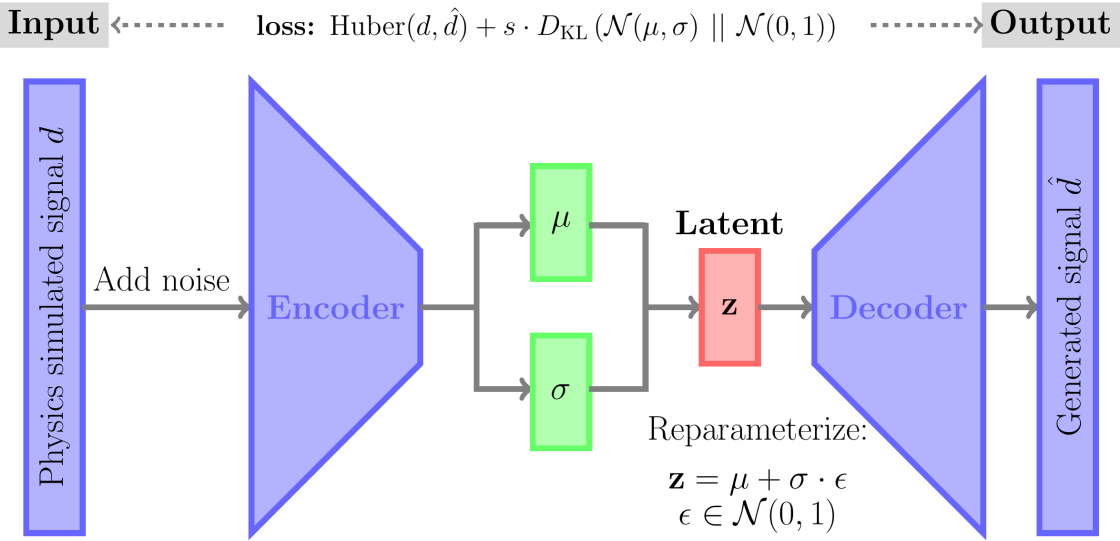
\includegraphics[width=\columnwidth]{../figures/fig1.png}
%		\caption{The architecture of a variational autoencoder.
%		}
%		\label{FIG:MODEL_VAE}
%	\end{figure}

	\subsection{Multi-Band Multi-Shot DWI Acquisition \& Modeling} \label{SEC:FWD}

	Our previous work \cite{tan_2024_naviepi} demonstrated
	the joint $k$-$q$-slice forward operator
	for multi-band multi-shot navigator-based interleaved EPI (NAViEPI) DWI acquisition.
	This operator can be understood as
	an extended sensitivity encoding (SENSE) operator \cite{pruessmann_2001_gsense},
	which maps the multi-slice multi-diffusion-weighted images ($\mathbf{\tilde{x}}$)
	to their corresponding $k$-space,
	\begin{equation}
		\mathcal{A}(\mathbf{\tilde{x}}) = \mathbf{P \Sigma \Theta F S \Phi} \mathbf{\tilde{x}}
		\label{EQU:FWD}
	\end{equation}
	Here, the images $\mathbf{\tilde{x}}$ are point-wise multiplied
	with the pre-computed shot-to-shot phase variation maps ($\mathbf{\Phi}$)
	and coil sensitivity maps ($\mathbf{S}$).
	The output images are then converted to $k$-space
	via two-dimensional fast Fourier transform ($\mathbf{F}$),
	point-wise multiplied with the multi-band phases ($\mathbf{\Theta}$),
	summed along the slice dimension ($\mathbf{\Sigma}$),
	and then multiplied by the $k$-space undersampling mask ($\mathbf{P}$).

	In \cref{EQU:FWD}, one challenge is
	to accurately estimate the shot-to-shot phase variation.
	Multiplexed sensitivity-encoding (MUSE) type reconstruction techniques
	\cite{liu_2004_diff_spiral,uecker_2009_nlinv_diff,chen_2013_muse,merrem_2019_nl_steam}
	realized the self-gating strategy,
	where the $k$-space data of each shot was used to reconstruct
	its corresponding shot image followed by a phase smoothing approach.
	Self-gated shot phase estimation does not require
	the acquisition of phase navigator data.
	However, it requires marginal undersampling factors per shot and
	fully-sampled DWI acquisition assembling all shots.
	Alternatively, undersampled DWI acquisition can be enabled
	via the acquisition of navigators for shot phase estimation
	\cite{tan_2024_naviepi}.
	This approach allows for mesoscale-resolution DWI at \SI{7}{\tesla},
	but still needs long scan time.
	As listed in \cref{TAB:ACQ}, the total acquisition of
	Protocol \#3 at \SI{0.7}{mm} isotropic resolution
	takes $16:27$ minutes with phase navigators.
	This scan time can be reduced to approximately 10 minutes
	be removing the phase navigators (Protocol \#4 in \cref{TAB:ACQ}).
%	However, as mentioned above, self gating poses a constraint
%	on the achievable undersampling factor
%	for parallel imaging and compressed sensing reconstruction methods
%	(e.g., MUSE and joint reconstruction with LLR regularization).

	With the operator $\mathcal{A}$, the joint reconstruction is expressed as,
	\begin{equation}
		\argmin_{\mathbf{\tilde{x}}} \norm{\mathbf{y} - \mathcal{A}(\mathbf{\tilde{x}})}_2^2 + \lambda \mathcal{R}(\mathbf{\tilde{x}})
		\label{EQU:INV}
	\end{equation}
	where $\mathbf{y}$ is the measured $k$-space data.
	The first term in \cref{EQU:INV} presents data consistency, and
	the second term presents the regularization function $\mathcal{R}(\tilde{x})$
	with the regularization strength $\lambda$.
	When using the Tikhonov regularization,
	i.e.~$\mathcal{R}(\mathbf{\tilde{x}}) = \norm{\mathbf{\tilde{x}}}_2^2$,
	\cref{EQU:INV} can be solved via the conjugate gradient (CG) method.
	For nonlinear regularization functions,
	such as the locally-low rank (LLR) regularzation \cite{tan_2024_naviepi} or
	neural networks with nonlinear activation functions,
	ADMM was employed in this work to solve for \cref{EQU:INV}.

%	\subsection{Variational Autoencoder (VAE)}
%
%	Autoencoders comprise an encoder and a decoder, connected through a latent space.
%	Conventional autoencoders have no regularization
%	on the latent space.
%	Consequently, the learned latent space lacks meaningful
%	and structural representation.
%	To allow for dimension reduction while keeping the major part of
%	the data structure,
%	Kingma and Welling \cite{kingma_2014_vae} proposed
%	the variational autoencoder (VAE), as shown in \cref{FIG:MODEL_VAE}.
%	In VAE, the encoder maps each diffusion-weighted signal
%	into a Gaussian distribution ($\mathcal{N}(\mu, \sigma)$) within the latent space.
%	The latent variable ($\mathbf{z}$) is sampled according to the encoded distribution.
%	The decoder then maps the latent variable to the input space.
%	The training of a VAE uses the Huber loss together
%	with the Kullback-Leibler Divergence (KL-D).
%	The Huber loss minimizes the difference between the input and the output,
%	whereas KL-D minimizes the approximate posterior in latent space and
%	the exact posterior (assumed to be Gaussian distribution).


	\subsection{Algorithm Unrolling for Deep Image Reconstruction}

	Algorithm unrolling has been an emerging technique
	in solving inverse problems with learnable deep neural networks.
	Algorithm unrolling consists of two ingredients.
	First, it uses deep neural networks to learns regularization function.
	Second, it is constrained
	by the data-consistency term.
	In other words,
	the forward pass of the estimate $\mathcal{A} (\mathbf{\tilde{x}})$
	must be close to the measured data $\mathbf{y}$.
	By mapping the operations used in iterative algorithms
	onto networks, unrolled algorithms can be trained with data,
	leading to much faster inference
	than conventional iterative algorithms \cite{monga_2021_algunroll}.
	Further, recent developments have shown that
	the operations used in compressed sensing MRI,
	i.e., sparsifying transformation and soft thresholding,
	can be learned via neural networks.
	For instance, Hammernik et al.~\cite{hammernik_2018_varnet}
	proposed to unroll the gradient descent algorithm
	with a learned neural network
	(e.g.~U-net \cite{ronneberger_2015_unet})
	as the regularization function.
	Aggarwal et al.~\cite{aggarwal_2018_modl} proposed
	the model-based deep learning architecture for inverse problems (MoDL)
	to unroll the alternating minimization algorithm
	with a learned residual denoising network \cite{he_2016_resnet}
	as regularization.

	% \subsubsection{Variational Network (VarNet)}
	% The unrolling update rule in VarNet \cite{hammernik_2018_varnet} reads
	% \begin{equation} \label{EQU:VarNet_Upd}
	% 	\left\{\begin{aligned}
	% 		\mathbf{z}^{(k)} &= \mathbf{\tilde{x}}^{(k)} - \lambda \cdot \mathcal{A}^H \Big( \mathcal{A} (\mathbf{\tilde{x}}^{(k)}) - \mathbf{y} \Big) \\
	% 		\mathbf{\tilde{x}}^{(k+1)} &= \mathbf{z}^{(k)} - \mathcal{N}_{\theta} (\mathbf{z}^{(k)})
	% 	\end{aligned}\right.
	% \end{equation}
	% with $k$ being the iteration (cascade) step.
	% The regularization is given as a neural network $\mathcal{N}_\theta$.
	% To learn the parameters $\theta$ and the gradient step size $\lambda$,
	% the loss function in VarNet is
	% \begin{equation}
	% 	\argmin_{(\theta, \lambda)} \mathcal{L} (\mathbf{x}_{\text{ref}}, \mathbf{\tilde{x}}^{(K)}) = \norm{\mathbf{\tilde{x}}^{(K)} - \mathbf{x}_{\text{ref}}}_2^2
	% 	\label{EQU:VarNet_Loss}
	% \end{equation}
	% where $\mathbf{\tilde{x}}^{(K)}$ is the estimate after $K$ iterations,
	% and $\mathbf{x}_{\text{ref}}$ denotes fully-sampled reference images.

	% \subsubsection{Model-based deep learning architecture for inverse problems (MoDL)}
	% MoDL \cite{aggarwal_2018_modl} tends to learn a denoising regularization,
	% and redefines \cref{EQU:INV} as
	% \begin{equation}
	% 	\argmin_{\mathbf{\tilde{x}}} \norm{\mathbf{y} - \mathcal{A}(\mathbf{\tilde{x}})}_2^2 + \lambda \norm{ \mathbf{\tilde{x}} - \mathcal{D}_{\omega}(\mathbf{\tilde{x}}) }_2^2
	% 	\label{EQU:DINV}
	% \end{equation}
	% which is solved by the alternating minimization,
	% \begin{equation} \label{EQU:MoDL_Upd}
	% 	\left\{\begin{aligned}
	% 		\mathbf{z}^{(k)} &= \mathcal{D}_{\omega} (\mathbf{\tilde{x}}^{(k)}) \\
	% 		\mathbf{\tilde{x}}^{(k+1)} &= \argmin_{\mathbf{x}} \norm{\mathbf{y} - \mathcal{A}(\mathbf{x})}_2^2 + \lambda \norm{ \mathbf{x} - \mathbf{z}^{(k)} }_2^2
	% 	\end{aligned}\right.
	% \end{equation}
	% where the second minimization problem is solved by CG.
	% MoDL shares weights among iterations, and thus the loss function reduces to
	% only one set of model parameters.
	% Both VarNet and MoDL require reference images,
	% and thus fall into the category of supervised learning.

	% In practice, it is challenging to acquire fully-sampled reference images.
	% To enable deep neural network training without fully sampled reference data,
	% Yaman et al.~\cite{yaman_2020_ssdu} proposed self-supervised learning via data undersampling (SSDU).
	% In SSDU, the undersampled data is partitioned into two disjoint sets,
	% one for the data-consistency term, and another for the loss function calculation.
	% Thus, the sampling mask $\mathbf{P}$ splits,
	% \begin{equation}
	% 	\mathbf{P} = \Theta ~\cup~ \Lambda
	% \end{equation}
	% SSDU follows the alternating update scheme in MoDL,
	% and such a splitting leads to two modifications in training.
	% First, the $k$-space data and the forward model in \cref{EQU:MoDL_Upd} is masked as
	% $\mathbf{y}_{\Theta}$ and $\mathcal{A}_{\Theta}$, respectively.
	% Second, the loss function is computed in $k$-space,
	% \begin{equation}
	% 	\argmin_{(\theta, \lambda)} \mathcal{L} (\mathbf{y}_{\Lambda}, \mathcal{A}_{\Lambda}(\mathbf{\tilde{x}}^{(K)}))
	% 	\label{EQU:SSDU_Loss}
	% \end{equation}
	% where a normalized $\ell_1$-$\ell_2$ loss is used \cite{yaman_2020_ssdu}.
	% Further, Yaman et al.~\cite{yaman_2022_zs} proposed subject-specific zero-shot learning,
	% where one single scan data is partitioned into three disjoint sets,
	% two used to enforce data consistency and to update loss,
	% and the last served as self-validation to allow for early stopping.

	% The regularization function in \cref{EQU:INV} can be nonlinear,
	% e.g.~the sparsity \cite{lustig_2007_cs} or the low-rankness \cite{liang_2007_psf} constraint.
	% In this scenario, algorithms such as
	% the fast iterative shrinkage thresholding (FISTA) \cite{beck_2009_fista}
	% and the alternating direction method of multipliers (ADMM) \cite{boyd_2010_admm}
	% are often employed.
	% These algorithms consist of a substep that transforms $\mathbf{\tilde{x}}$
	% to a sparsifying domain or a specialized matrix format
	% (e.g., the spatial-diffusion matrix in our previous work \cite{tan_2024_naviepi})
	% and then performs nonlinear thresholding to promote sparsity or low-rankness.
	% This substep shares similarities to deep neural networks,
	% and inspires the seminal work on algorithm unrolling
	% by Gregor and LeCun \cite{gregor_2010_algunroll}.
	% Instead of a hand-crafted regularization function,
	% algorithm unrolling learns deep \textit{prior}
	% via the use of deep neural networks as the regularization function.
	% This enables the learning of true image \textit{prior} during the training process
	% and much faster inference than iterative reconstruction with hand-crafted regularization functions.
	% An excellent review of algorithm unrolling
	% has been provided by Monga et al.~\cite{monga_2021_algunroll}.

	% In the area of image reconstruction for accelerated MRI,

	\subsection{Self-Supervised Learning for Image Reconstruction}

	In many MRI applications, such as dynamic imaging and diffusion-weighted imaging
	acquiring fully-sampled data
	for supervised learning can be challenging.
	To tackle this issue, Yaman et al.~\cite{yaman_2020_ssdu}
	proposed self-supervised learning via data undersampling (SSDU),
	which learns the regularization function in \cref{EQU:INV}
	by splitting available undersampled data into two disjoint sets,
	one of which is used in the data consistency term and
	another used for the computation in the training loss function.
	The training of SSDU requires large undersampled data sets.
	To close the domain gap between training and test data,
	Yaman et al.~\cite{yaman_2022_zs} proposed
	scan-specific zero-shot self-supervised learning (ZSSSL),
	which splits a single data set into three disjoint sets
	for (a) the data consistency term, (b) the loss calculation during training,
	and (c) validation, respectively.
	Recently, ZSSSL has been adopted for multi-contrast image reconstruction
	\cite{heydari_2024_jmaple}.

	% ============================== %
	\section{Methods}

	\newcolumntype{a}{p{0.30\textwidth}}
	\newcolumntype{b}{p{0.22\textwidth}}
	\begin{table*}
		\centering
		\caption{iEPI with or without navigators acquisition protocols}
		\label{TAB:ACQ}
		\begin{tabular}{a | b b}
			\toprule
			\textbf{Protocol} & \textbf{\#1} \;\;\; / \;\;\; \textbf{\#2} & \textbf{\#3} \\
			\hline
			Diffusion mode & \multicolumn{2}{c}{MDDW} \\
			Diffusion scheme & \multicolumn{2}{c}{monopolar} \\
			Diffusion direction & $20$ & $114$ \\
			$b$-value (\si{s/mm^2}) & $1000$ & 3-shell \\
			$b_0$ & $1$ & $12$ \\
			FOV (\si{\square\mm}) & \multicolumn{2}{c}{$200$} \\
			Matrix size & $286 \times 286$ & $200 \times 200$ \\
			In-plane resolution (\si{\square\mm}) & $0.7 \times 0.7$ & $1.0 \times 1.0$ \\
			Slice thickness (\si{\mm}) & $0.7$ & $1.0$ \\
			Slices & $176$ & $114$ \\
			Navigator & Yes \;\;\; / \;\;\; No & No \\
			Shots & $3$ & $2$ \\
			TR (\si{\ms}) & $15000$ \;\;\; / \;\;\; $8900$ & $4900$ \\
			TE (\si{\ms}) & $58/98.3$ \;\;\; / \;\;\; $58$ & $70$ \\
			ESP (\si{\ms}) & $1.17$ & $1.02$ \\
			Bandwidth (\si{Hz/Pixel}) & $972$ & $1086$ \\
			Partial Fourier & $5/8$ & $6/8$ \\
			Acceleration & $2 \times 2$ & $3 \times 3$ \\
			Acquisition (\si{\minute}) & $16:27$ \;\;\; / \;\;\; $9:57$  & $20:55$ \\
			\bottomrule
		\end{tabular}
	\end{table*}

	\subsection{Data Acquisition}

	\cref{TAB:ACQ} lists three acquisition protocols implemented on
	a clinical \SI{7}{\tesla} MR system
	(MAGNETOM Terra, Siemens Healthineers, Erlangen, Germany)
	with a 32-channel head coil (Nova Medical, Wilmington, MA, USA)
	and the XR-gradient system
	(maximum gradient strength \SI{80}{\milli\tesla/\meter} and
	a peak slew rate \SI{200}{\tesla/\meter/\second}).
	Protocols \#1 and \#2 realized mesoscale DWI with \SI{0.7}{mm}
	isotropic resolution. Two-fold acceleration was employed
	in both in-plane and slice directions.
	Every DWI was acquired by three shots in an interleaved manner,
	which resulted in $6 \times 2$-fold acceleration per shot.
	Noteworthy, the total scan time can be reduced to about 10~minutes
	(Protocol \#2) when switching off navigator acquisition.
	\hl{Protocol \#3} realized three-shell diffusion acquisition
	with $b$-values spanning $1000$, $2000$, and $3000$~\si{s/mm^2}
	at \SI{1.0}{mm} isotropic resolution.
	Four young healthy volunteers with written informed consent
	approved by the local ethics committee
	participated in this study.


%	\subsection{Image Reconstruction with a Learned VAE as regularization}
%
%	To learn a VAE model as shown in \cref{FIG:MODEL_VAE},
%	we fed the VAE with diffusion-weighted signal simulated
%	with the diffusion tensor model \cite{basser_1994_dmri} and
%	the employed $b$-value and diffusion-encoding vectors in data acquisition.
%	The signal was augmented with added Gaussian noise and passed through the VAE network.
%	The training loss function was defined as the sum of the Huber and and KL-D function
%	between the simulated signal and the output of VAE.
%
%	In this work, both the encoder and the decoder in VAE consisted of
%	4 fully-connected linear layers.
%	The last layer in the decoder used the sigmoid activation function,
%	whereas the other layers used the ReLU activation function.
%	The latent signal had 6 features,
%	the same as the Gaussian distribution parameters $\mu$ and $\sigma$.
%	The output features of each encoder layer gradually decreased
%	from the number of features in simulated signal
%	to the number of features in latent signal,
%	whereas the input features of each decoder layer gradually increased
%	from the number of features in latent signal to the number of features in simulated signal.
%	After training, the VAE model was used as the regularization function in \cref{EQU:INV},
%	which was solved by ADMM in a plug-and-play manner.

	\subsection{Image Reconstruction via ADMM Unrolling and Zero-Shot Self-Supervised Learning}

	\begin{algorithm}
		\caption{ADMM Unrolling for ZSSSL} \label{ALG:ADMM}
		\begin{algorithmic}[1]
			\State \textbf{Initialization}:
			\State \;\; split sampling mask $\mathbf{P}$ into 12 repetitions, each of which consists of three disjoint sets $\mathbf{T}$, $\mathbf{L}$, and $\mathbf{V}$
			\State \;\: $p \gets 0$ and $N_{\mathrm{epoch}} \gets 100$
			\State \;\; $\mathcal{D}_{\omega}$ set as ResNet
			\State \;\; $\rho \gets 0.05$ and $\lambda \gets 0.05$
			\State \;\; $\mathrm{Loss}_{\mathrm{valid}} \gets \inf$ and $\mathrm{trace} \gets 0$
			\Function{ADMM}{$\mathrm{mask}$}
			\State $\mathcal{A}_\mathrm{mask} \gets$ set the mask in the forward operator $\mathcal{A}$
			\State $\tilde{\mathbf{x}}^{(0)} \gets \mathcal{A}_\mathrm{mask}^H (\mathbf{y})$
			\State $\mathbf{v}^{(0)} \gets \tilde{\mathbf{x}}^{(0)}$ and $\mathbf{u}^{(0)} \gets \mathbf{0}$
			\State $k \gets 0$ and $N_{\mathrm{unroll}} \gets 8$
			\While{$k < N_{\mathrm{unroll}}$}
			\State $\tilde{\mathbf{x}}^{(k+1)} \gets $ conjugate gradient with 6 iterations
			\State $\mathbf{v}^{(k+1)} \gets (\lambda/\rho) \cdot \mathcal{D}_{\omega} (\mathbf{\tilde{x}}^{(k+1)} + \mathbf{u}^{(k)})$
			\State $\mathbf{u}^{(k+1)} \gets \mathbf{u}^{(k)} + \mathbf{\tilde{x}}^{(k+1)} - \mathbf{v}^{(k+1)}$
			\State $k \gets k+1$
			\EndWhile
			\State \Return $\tilde{\mathbf{x}}^{(k+1)}$
			\EndFunction
			\State \textbf{Training}:
			\While{$p < N_{\mathrm{epoch}}$ or $\mathrm{trace} \leq 12$}
			\State $\mathbf{x}_t \gets \mathrm{ADMM}(\mathbf{T})$
			\State $\mathrm{Loss}_{\mathrm{train}} \gets \mathcal{L}(\mathbf{L} \mathbf{y}, \mathcal{A}_\mathbf{L}(\mathbf{x}_t))$
			\State update $\omega$ via ADAM
			\State \textbf{Validation}:
			\State $\mathbf{x}_t \gets \mathrm{ADMM}(\mathbf{T} \cup \mathbf{L})$
			\State $\mathrm{Loss}_{\mathrm{temp}} \gets \mathcal{L}(\mathbf{V} \mathbf{y}, \mathcal{A}_\mathbf{V}(\mathbf{x}_t))$
			\If{$\mathrm{Loss}_{\mathrm{temp}} \leq \mathrm{Loss}_{\mathrm{valid}}$}
			\State $\mathrm{Loss}_{\mathrm{valid}} \gets \mathrm{Loss}_{\mathrm{temp}}$
			\State $\mathrm{trace} \gets 0$
			\Else
			\State $\mathrm{trace} \gets \mathrm{trace} + 1$
			\EndIf
			\EndWhile
		\end{algorithmic}
	\end{algorithm}

	\begin{figure}
		\centering
		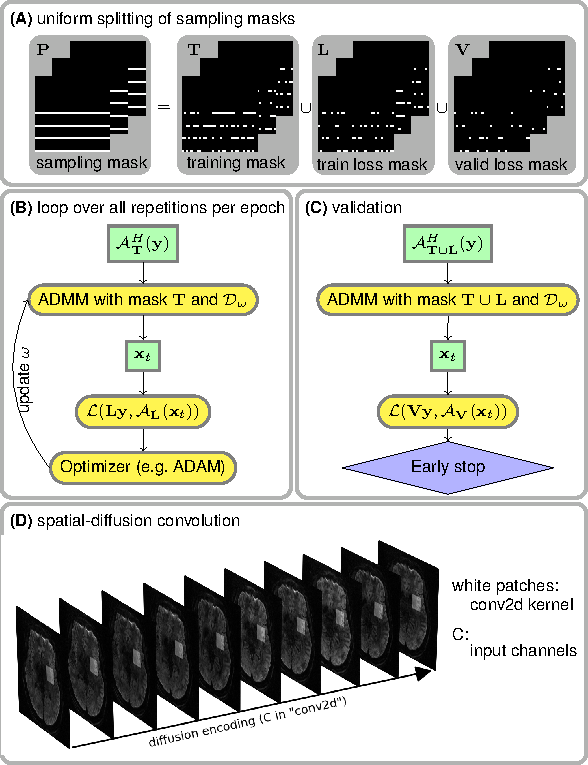
\includegraphics[width=\columnwidth]{../figures/fig1.pdf}
		\caption{Illustration of the key components in ZSSSL.
			\textbf{(A)} The sampling mask $P$ in \cref{EQU:FWD} was
			uniformly split into three disjoint sets:
			the training mask $\mathbf{T}$ used for
			the data consistency term during ZSSSL training,
			the train loss mask $\mathbf{L}$ used for
			the loss function calculation during ZSSSL training, and
			the validation loss mask $\mathbf{V}$ used for
			the loss function calculation during ZSSSL validation.
			\textbf{(B)} and \textbf{(C)} show the flowchart
			for the training and the validation of ZSSSL, respectively.
			Note that the ResNet parameters $\omega$ are updated during training,
			but remain fixed during the validation step.
			\textbf{(D)} A stack of DWIs is input into ResNet during ADMM unrolling.}
		\label{FIG:ZSSSL}
	\end{figure}

	Instead of the two-step alternating minimization unrolling scheme as used in MoDL
	\cite{aggarwal_2018_modl},
	we employed the ADMM unrolling
	to solve the self-supervised learning reconstruction
	in \cref{EQU:INV}. The update rule of ADMM unrolling reads
	\begin{equation} \label{EQU:ADMM}
		\left\{\begin{aligned}
			\mathbf{\tilde{x}}^{(k+1)} &= \argmin_{\mathbf{x}} \norm{\mathbf{y} - \mathcal{A}(\mathbf{x})}_2^2 + \rho/2 \norm{ \mathbf{x} - \mathbf{v}^{(k)} + \mathbf{u}^{(k)}}_2^2 \\
			\mathbf{v}^{(k+1)} &= (\lambda/\rho) \cdot \mathcal{D}_{\omega} (\mathbf{\tilde{x}}^{(k+1)} + \mathbf{u}^{(k)}) \\
			\mathbf{u}^{(k+1)} &= \mathbf{u}^{(k)} + \mathbf{\tilde{x}}^{(k+1)} - \mathbf{v}^{(k+1)}
		\end{aligned}\right.
	\end{equation}
	ADMM updates the variables $\mathbf{\tilde{x}}$, $\mathbf{v}$,
	and $\mathbf{u}$ in an alternating scheme.
	It splits the unrolled reconstruction into three steps,
	as shown in \cref{EQU:ADMM} and in the pseudo code of \cref{ALG:ADMM}.
	First, the updating step for $\mathbf{\tilde{x}}$ is solved by conjugate gradient.
	Second, the variable $\mathbf{v}$ is then updated
	via the forward pass of the neural network $\mathcal{D}_{\omega}$
	with the input as the sum of current estimates
	of $\mathbf{\tilde{x}}$ and $\mathbf{u}$.
	Third, the variable $\mathbf{u}$ is updated
	by adding its current estimate to the difference
	between $\mathbf{\tilde{x}}$ and $\mathbf{v}$.

	As shown in \cref{FIG:ZSSSL}, the data sampling mask $\mathbf{P}$
	in ZSSSL \cite{yaman_2022_zs} is split into
	three disjoint sets, the training mask $\mathbf{T}$ for the data consistency term,
	the training loss mask $\mathbf{L}$ for the loss function calculation,
	and the validation loss mask $\mathbf{V}$.
	Each set consists of 12 repetitions constructed via random uniform sampling
	of the data mask $\mathbf{P}$.
	In each training epoch, every repetition is looped through
	in order to update the ResNet parameters $\omega$.
	Plus, the validation step is performed after every training epoch
	to update the minimal validation loss.
	If the validation loss does not reduce for 12 consecutive epochs or
	if 100 epochs are reached, the training is terminated.

	The index $k$ in \cref{EQU:ADMM} denotes the unrolling iteration,
	and $\mathcal{D}_{\omega}$ denotes the residual network (ResNet) \cite{he_2016_resnet}
	parameterized by $\omega$.
	In this work, 2D convolution was employed to construct the ResNet.
	In PyTorch, 2D convolution requires four-dimensional tensors as input and output.
	For instance, a matrix with the size $(N, C, H, W)$ is acceptable
	for the the 'conv2d' function in PyTorch.
	Here, $W$ and $H$ denote the width and height of the convolution kernel,
	$C$ denotes the number of channels, and $N$ denotes the batch size.
	However, the DWIs ($\tilde{x}$) to be reconstructed
	has the size $(N_{\text{diff}}, N_Z, N_Y, N_X, 2)$,
	where $2$ stands for the real and imaginary part of the complex-valued DWIs,
	$N_X$ and $N_Y$ are the width and the height of DWIs,
	$N_Z$ is the number of slices (same as the multi-band factor), and
	$N_{\text{diff}}$ is the number of diffusion encodings.
	To train a ResNet based on 2D convolution, the DWIs were reshaped and permuted
	as $(N_Z, 2 \cdot N_{\text{diff}}, N_Y, N_X)$, as illustrated in \cref{FIG:ZSSSL} (D).
	In this manner, 2D convolution kernels in combination with ReLU activation functions
	loop through the varying diffusion-weighted contrast
	to learn the key features of the high-dimensional data and
	to reduce noisy and aliasing artifacts in unrolled reconstruction.

	\subsection{Comparison of Regularization Techniques}

	This work compared the reconstruction performance
	of three different regularization techniques,
	Tikhonov $\ell^2$ regularization (as used in MUSE),
	LLR regularization,
	and ZSSSL with a learned regularization.
	Note that MUSE is a simultaneous multi-slice (SMS) parallel imaging method
	and poses no regularization along the diffusion dimension,
	effectively solving each DWI reconstruction independently.
	In contrast, all other regularized reconstructions
	fall into the joint reconstruction regime.
	They jointly reconstruct all DWIs
	and imposes regularization terms that explore spatial-diffusion redundancy.
	For example, LLR enforces low rankness of
	local spatial-diffusion matrices from DWIs,
	whereas ZSSSL learns a ResNet regularization function
	based on spatial-diffusion convolution kernels
	while enforcing data consistency during the unrolled training process.

	\subsection{Self-Gated ZSSSL}

	As discussed in \cref{SEC:FWD}, there are two approaches for
	estimating shot-to-shot phase variation: self-gated and navigator-based.
	The self-gated approach, as used in MUSE \cite{chen_2013_muse},
	requires fully-sampled DWI acquisition and
	has typically reported only a small number of shots (up to 4).
	The previously proposed NAViEPI approach enabled high-resolution DWI
	with the use of undersampled iEPI and shot-to-shot phase navigator acquisition.
	While NAViEPI results in shorter scan time than fully-sampled iEPI,
	the use of phase navigator still elongates the acquisition,
	as listed in \cref{TAB:ACQ}.
	Therefore, a key question is whether it would be feasible to
	discard phase navigator while keeping undersampled iEPI acquisition.
	In this work, we investigated the feasibility of ZSSSL in self-gated scan
	for \SI{0.7}{\milli\meter} isotropic resolution DWI.

	\subsection{ZSSSL Model Generalization} \label{SEC:ZSSSL_GEN}

	\hl{We evaluated the generalization of the ZSSSL model in two aspects.}
	First, using the 4-shot fully-sampled data acquired by
	Protocol \#1 \cref{TAB:ACQ}, we trained ZSSSL with all 4 shots
	and then tested the trained model with retrospectively undersampled 2-shot data.
	Second, with the \SI{0.7}{\milli\meter} isotropic resolution DWI data
	containing 88 multi-band slices acquired from Protocol \#3 in \cref{TAB:ACQ},
	we trained the ZSSSL with only one slice and
	then performed the inference reconstruction on the remaining slices.

	% \subsection{Latent Space Embedded Zero-Shot Learning}

	% ZSSSL partitions the undersampled data into three sets,
	% so the sampling mask ($\mathbf{P}$) becomes
	% $\mathbf{P} = \mathbf{P}_1 \cup \mathbf{P}_2 \cup \mathbf{P}_3$.
	% Here, $\mathbf{P}_1$ is used for the data consistency term
	% during training,
	% which modifies the $\mathbf{\tilde{x}}$ update step
	% in \cref{EQU:ADMM} as
	% $\mathbf{\tilde{x}}^{(k+1)} = \argmin_{\mathbf{x}} \norm{\mathbf{P}_1 \mathbf{y} - \mathbf{P}_1 \mathcal{A}(\mathbf{x})}_2^2 + \rho/2 \norm{ \mathbf{x} - \mathbf{v}^{(k)} + \mathbf{u}^{(k)}}_2^2$.
	% Given the estimated $\mathbf{\tilde{x}}$,
	% $\mathbf{P}_2$ is then used to define the training loss function:
	% \begin{equation}
	%     \label{EQU:LOSS}
	%     \mathcal{L}(\mathbf{P}_2 \mathbf{y}, \mathbf{P}_2 \mathcal{A}(\mathbf{\tilde{x}}))
	% \end{equation}
	% which is computed from
	% the mixed-$\ell^1$-$\ell^2$ norm of the two inputs
	% \cite{yaman_2020_ssdu}.
	% $\mathbf{P}_3$ is used to compute the validation loss.
	% When the validation loss is consecutively smaller than
	% the training loss for 12 times,
	% the training process will be stopped.
	% After training, the undersampled data set is used for inference.

	\subsection{Computation}

	All reconstructions were in this work done on a single A100 SXM4/NVLink GPU
	with \SI{80}{\giga\byte} memory (NVIDIA, Santa Clara, CA, USA).
	Computing infrastructure was provided by
	the Erlangen National High Performance Computing Center.

	Note that the data from Protocol \#2 in \cref{TAB:ACQ} contains a total of
	126 diffusion-weighted images, which is too large for the LLR and the ResNet computation
	in a single A100 GPU. As a result, this data was uniformly
	split into three consecutive parts,
	with each part containing 42 diffusion-weighted images.

	% ============================== %
	\section{Results}

	\subsection{Retrospectively Self-Gated ZSSSL}

	\begin{figure*}
		\begin{minipage}[c]{0.75\textwidth}
			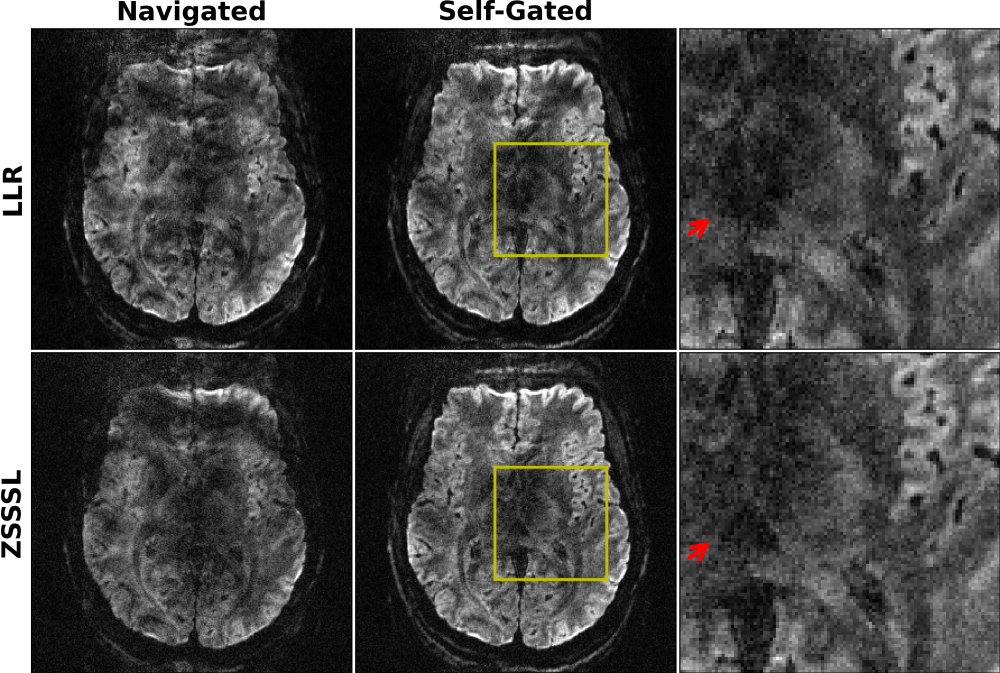
\includegraphics[width=\textwidth]{../figures/fig2.png}
		\end{minipage}\hfill
		\begin{minipage}[c]{0.23\textwidth}
			\caption{Comparison of (top) LLR regularized and (bottom) ZSSSL
				reconstruction on 0.7~mm isotropic resolution DWI
				acquired by Protocol \#1
				with shot phase estimated from
				(left) navigators and (middle) imaging echoes, respectively.
				Zoomed views of the yellow boxes from the self-gated reconstruction
				are displayed in the right column.
				The use of navigators prolongs the total scan time,
				and thus increases the sensitivity to motion,
				as shown in the single-direction DWI reconstructed
				with navigated shot phase.
				The retrospectively self-gated reconstruction discards navigators,
				and renders sharper DWI. Compared to LLR, ZSSSL is advantageous
				in resolving clearer tissue boundaries in DWI,
				as indicated by red arrows.}
				\label{FIG:MOTION_RETRO_TRA}
		\end{minipage}
	\end{figure*}

	\cref{FIG:MOTION_RETRO_TRA} demonstrates
	the efficacy of the self-gated ZSSSL reconstruction
	by comparing to the navigated reconstructions
	using the NAViEPI data of the first volunteer
	from Protocol \#1 in \cref{TAB:ACQ}.
	The diffusion encoding with accidental inter-shot motion
	reconstruction results were displayed.

	The selected DWIs showed residual aliasing-like and
	severe motion-blurring artifacts
	in the navigated reconstructions.
	The main reason of these artifacts is that
	the addition of navigator acquisition
	increased the total scan time,
	resulting in higher sensitivity to accidental inter-shot motion.
	Admittedly, navigators are valuable in the case of ultra high resolution
	using many shots, e.g.~3-fold in-plane undersampling and 5-shot acquisition
	for the in-plane resolution of 0.5~mm \cite{tan_2024_naviepi}.
	In this experiment, however, the utilization of 3 shots yielded
	$6 \times 2$-fold acceleration per shot (refer to Protocol \#3).
	Such an acceleration rate proved achievable in the self-gated approach,
	as demonstrated in the self-gated reconstruction results.
	The self-gated ZSSSL reconstruction largely reduced the residual aliasing
	and motion artifact.
	Further, self-gated ZSSSL exhibits much clearer tissue delineation
	in reconstructed DWIs, as indicated by red arrows in the zoomed-in views
	in \cref{FIG:MOTION_RETRO_TRA},
	whereas self-gated LLR suffers from
	blurry tissue boundaries and signal dropouts.

	\begin{figure*}
		\begin{minipage}[c]{0.75\textwidth}
			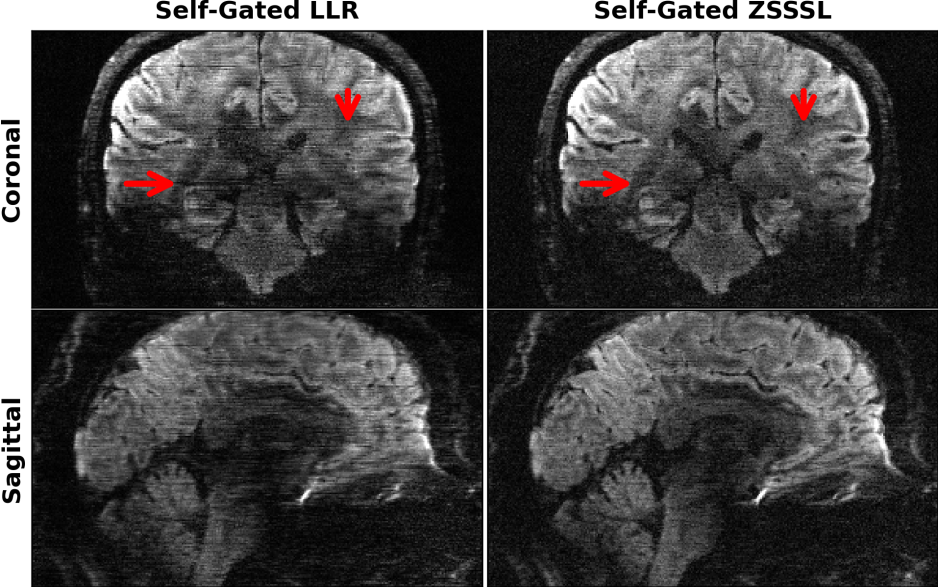
\includegraphics[width=\textwidth]{../figures/fig3.png}
		\end{minipage}\hfill
		\begin{minipage}[c]{0.23\textwidth}
			\caption{Single-direction DWI at 0.7~mm isotropic resolution
				as reconstructed by retrospectively self-gated
				(left) LLR and (right) ZSSSL
				in (top) the coronal and (bottom) the sagittal views.
				The same diffusion direction as in \cref{FIG:MOTION_RETRO_TRA}
				is chosen for display.
				ZSSSL reduces phase ambiguities in the shot-combined reconstruction
				, thereby rendering clearer tissue delineation and
				reduced stripping artifacts (as indicated by the red arrows).}
			\label{FIG:MOTION_RETRO_2}
		\end{minipage}
	\end{figure*}

	\cref{FIG:MOTION_RETRO_2} shows diffusion-weighted images
	at the same diffusion encoding as in \cref{FIG:MOTION_RETRO_TRA}
	in the coronal and the sagittal view, respectively.
	As mentioned in \cref{SEC:ZSSSL_GEN}, ZSSSL was trained using only one slice
	and then inferred on the remaining slices.
	The ZSSSL model generalized well across slices.
	The inference of every slice took only about 1~minute,
	whereas the LLR reconstruction took about 48~minutes per slice.
	More importantly, the self-gated LLR reconstruction exhibited residual
	motion-induced stripping artifacts
	in both coronal and sagittal views \cite{chang_2021_musium},
	whereas the self-gated ZSSSL approach substantially removed these artifacts
	and supplied high-quality DWI without the need of navigators.

	\subsection{Prospectively Self-Gated ZSSSL}

	\begin{figure*}
		\centering
		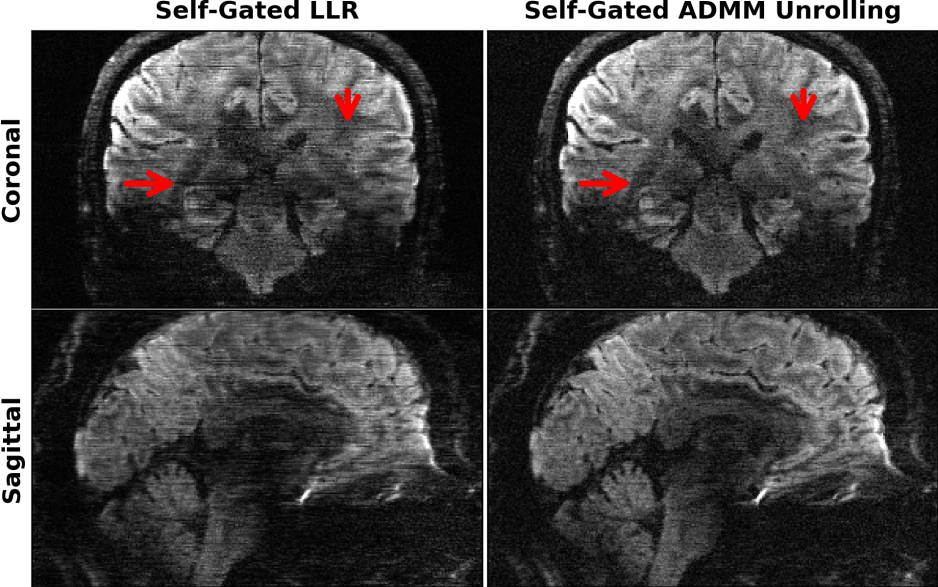
\includegraphics[width=\textwidth]{../figures/fig4.png}
		\caption{0.7~mm isotropic mesoscale DWI with 21 volumes at about 10~minutes
			without the acquisition of navigators.
			(A) Single-direction DWI and
			(B) Mean DWI of 20 diffusion directions
			at three orthogonal orientations are displayed.
			DWIs were reconstructed by
			(top) MUSE, (middle) LLR, and (bottom) ZSSSL.
			MUSE suffers from severe noise artifacts at such small voxel size.
			LLR is able to clean up most of the noise,
			but is still hampered by signal void artifacts in the axial view,
			which appears as stripping artifacts in coronal and sagittal views
			(as indicated by red arrows).
			ZSSSL significantly reduces both noise and signal voids.
			In the mean DWI images, LLR shows amplified noise
			in the cerebellum region,
			whereas ZSSSL yields more homogeneous signal distributions.}
		\label{FIG:MOTION_PROS}
	\end{figure*}

	\cref{FIG:MOTION_PROS} compares the reconstruction results
	using the prospectively acquired iEPI data without navigators
	of the second volunteer
	(refer to Protocol \#2 in \cref{TAB:ACQ}).
	The snapshot single diffusion-direction DWIs
	as well as mean DWIs
	at three orthogonal planes were displayed.
	The MUSE reconstruction suffered from strong noise
	at such high spatial resolution.

	The LLR regularized reconstruction largely reduced noise,
	but still exhibited signal void in the axial view,
	which appeared as striping artifacts in the coronal and sagittal views
	(refer to the red arrows in \cref{FIG:MOTION_PROS}).
	These artifacts can be reduced by incorporating adaptive noise estimation
	in LLR regularization \cite{cordero_2019_cplxdwi}.
	On the other hand, the LLR regularized reconstruction
	showed residual noise in the cerebellum region
	(refer to the blue arrows in \cref{FIG:MOTION_PROS}),
	which could be caused by the $B_1$ excitation field inhomogeneity
	at \SI{7}{\tesla}.

	The above-mentioned artifacts were nearly gone in the ZSSSL reconstruction.
	The DWI in the axial view showed clearer diffusion contrasts
	and thus better tissue delineation in the coronal and sagittal views.
	Plus, the DWI in the sagittal view showed more homogeneous
	signal distribution.

	\begin{figure}
		\centering
		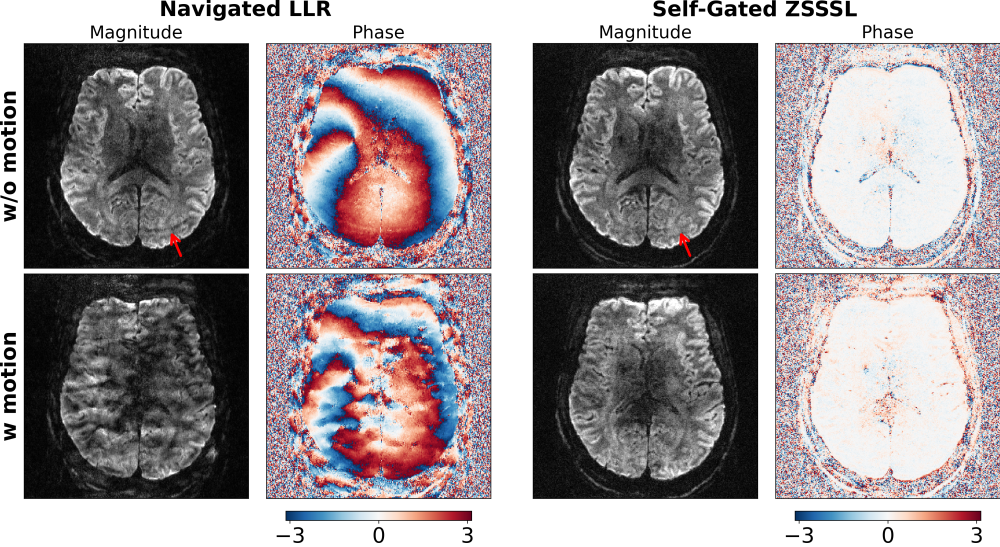
\includegraphics[width=\columnwidth]{../figures/fig5.png}
		\caption{Convergence analysis along the ADMM unrolling training
			and validation epochs
			for the ZSSSL results in \cref{FIG:MOTION_PROS}.
			Displayed curves are (red solid) the training loss,
			(red dashed) the validation loss,
			and (blue solid) the learned regularization strength $\lambda$, respectively.}
		\label{FIG:CONVERGENCE}
	\end{figure}

	\cref{FIG:CONVERGENCE} displays the training and validation loss
	as well as the learned regularization strength along epochs.
	It can be seen that 100 epochs were sufficient for
	the convergence of ADMM unrolling.
	In addition, the regularization strength converged
	to the value of about 0.027.


	\begin{figure*}
		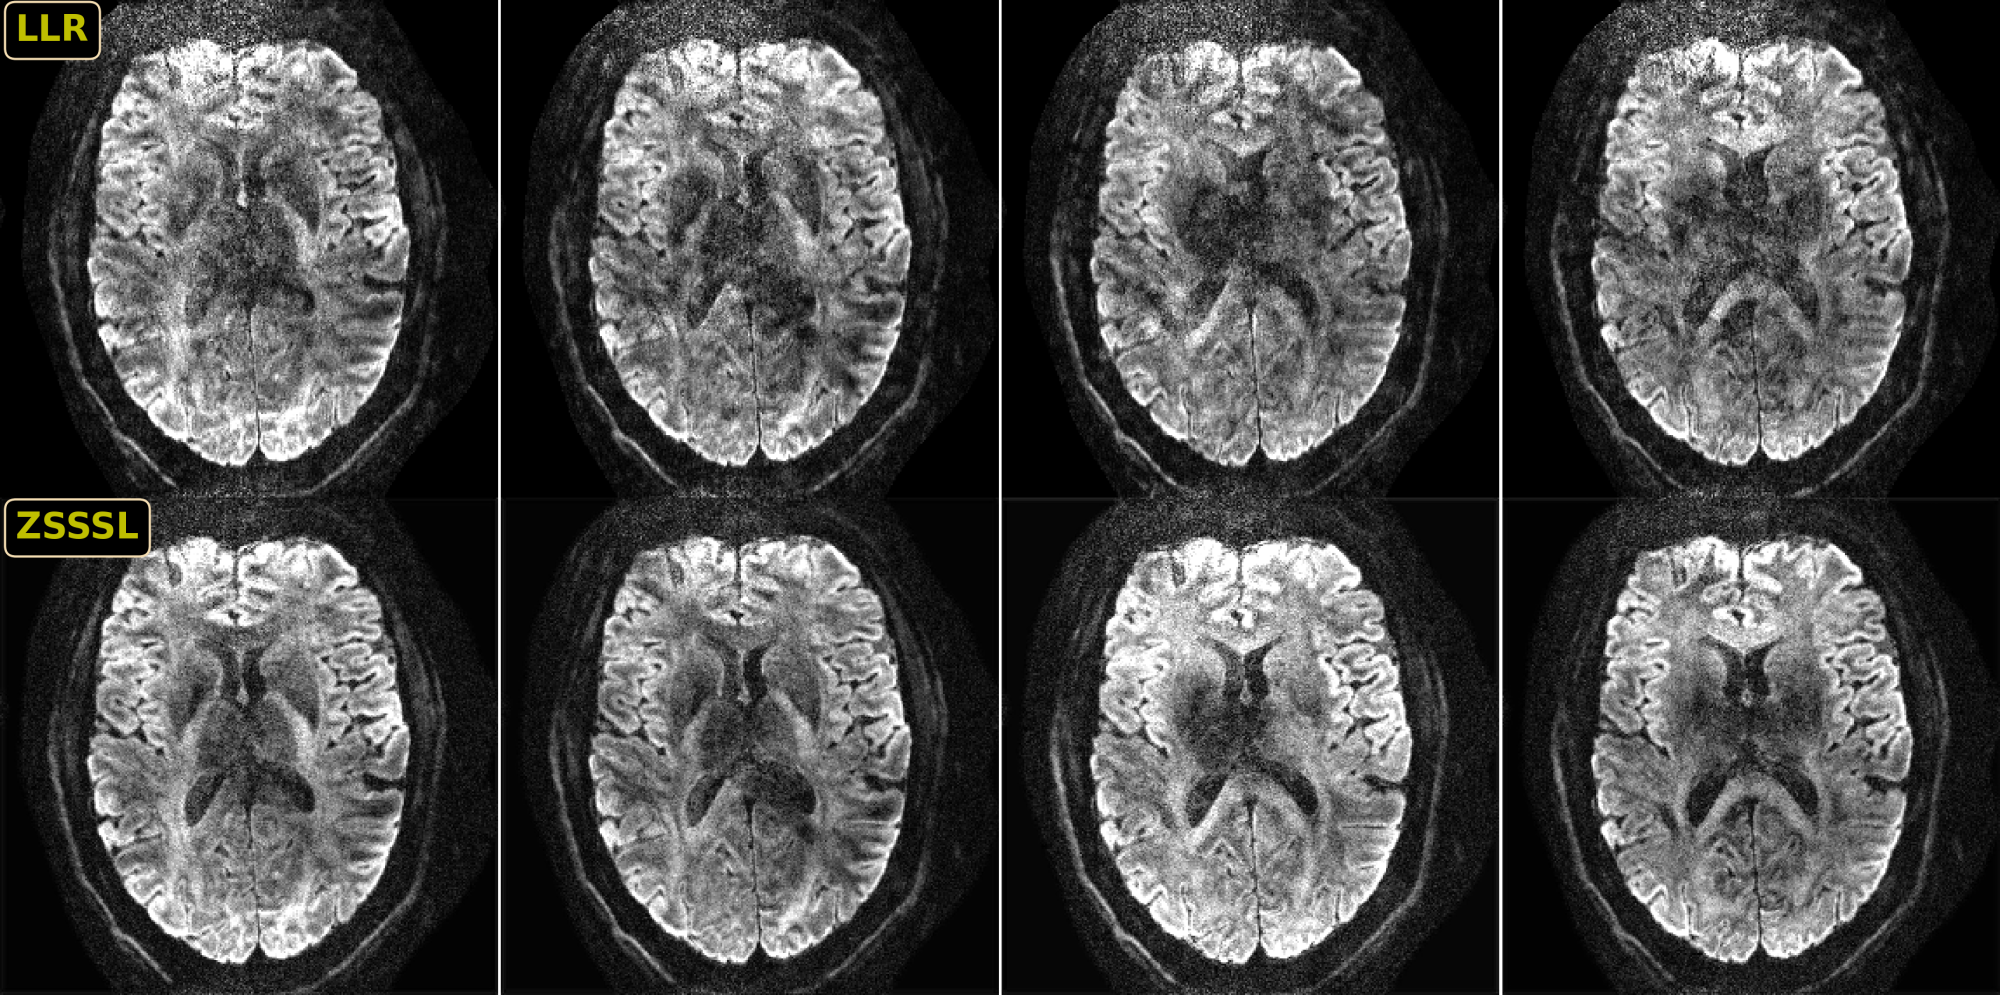
\includegraphics[width=\textwidth]{../figures/fig6.png}
		\caption{Prospectively self-gated DWI reconstruction results
			at 0.7~mm isotropic resolution. Displayed images are
			one axial slice at four different diffusion-encoding directions.
			ZSSSL enables much cleaner delineations of diffusion contrasts
			than LLR.}
		\label{FIG:SG_ZSSSL_VOL3}
	\end{figure*}

	\cref{FIG:SG_ZSSSL_VOL3} showed the reconstructed DWIs
	at four diffusion encodings based on the iEPI data
	acquired from the third volunteer.
	In this experiment, the volunteer was instructed
	to keep still during scan.
	Again, the proposed ZSSSL reconstruction
	with spatial-diffusion convolution illustrated
	superior tissue structure delineation
	to the LLR regularized reconstruction.

%	\cref{FIG:MOTION_RETRO_TRA} displays the regularized reconstruction results
%	using both the 4-shot fully-sampled iEPI data and
%	the retrospectively 2-shot undersampled iEPI data.
%	Firstly, compared to MUSE, all other regularized joint reconstructions
%	(LLR and ZSSSL)
%	demonstrated denoising capabilities in the case of 4-shot fully-sampled iEPI.
%	Secondly, when the 4-shot iEPI data was retrospectively undersampled to 2 shots,
%	the undersampling factor became $4 \times 3$
%	(4-fold in-plane undersampling and 3-fold slice undersampling).
%	As expected, the MUSE reconstruction showed increased noise.
%	In contrast, both LLR and ZSSSL reconstructions
%	showed strong denoising performance.
%	ZSSSL, in particular, provided sharper and clearer delineation
%	of brain tissues compared to LLR.
%	This may attribute to the fact that the same LLR regularization strength was used
%	for both the 4-shot and the 2-shot reconstructions.
%	While this empirically chosen regularization strength
%	was optimal for the 4-shot data,
%	it resulted in slightly blurring artifacts for the 2-shot data.
%	ZSSSL, on the contrary, learned the regularization strength
%	($\lambda$ in \cref{EQU:INV}) during training,
%	eliminating the need for empirical selection.
%	Moreover, note that the LLR reconstruction took about 40 minutes for the data,
%	whereas the training of ZSSSL required about 3 hours,
%	with inference taking only 1 minute.


	\subsection{DWI at $b$-Value of $3000$~\si{s/mm^2}}

	\begin{figure*}
		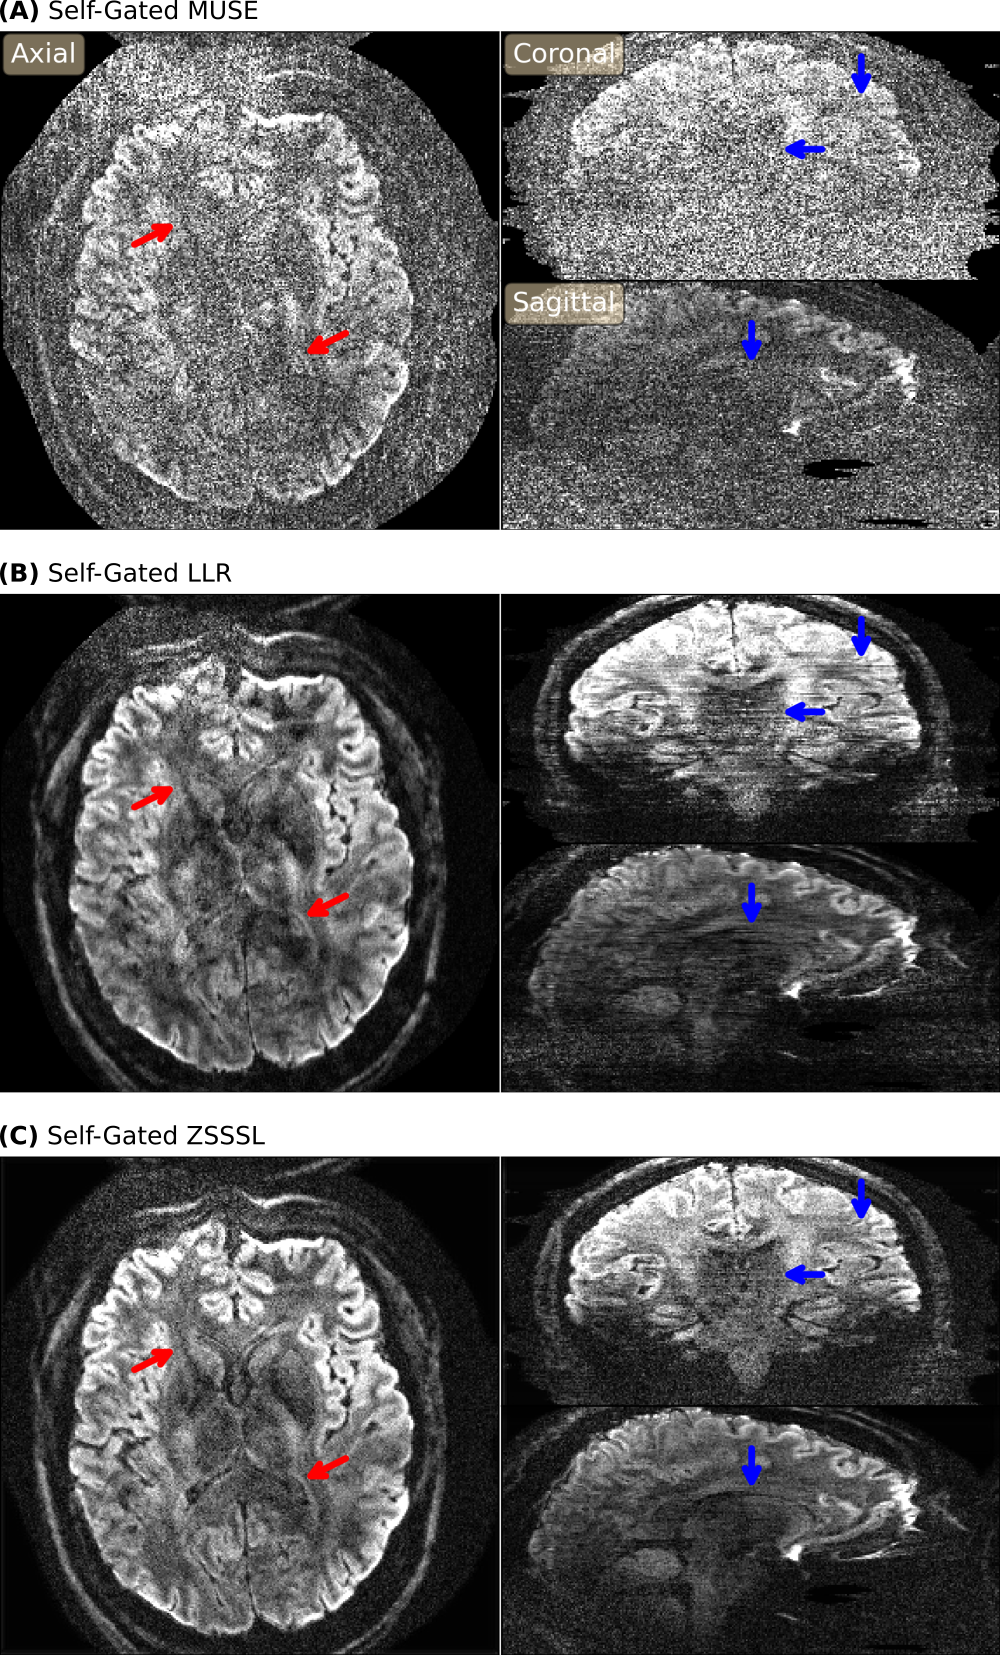
\includegraphics[width=\textwidth]{../figures/fig7.png}
		\caption{Reconstruction results of 3-shell \SI{1.0}{mm} isotropic resolution
			DWI with $3 \times 3$ acceleration: (left) LLR and (right) ZSSSL.
			(Top) Single-direction DWI at the $b$-values of
			\SI{3000}{s/mm^2} and
			(bottom) colored fractional anisotropy maps.}
		\label{FIG:B3000}
	\end{figure*}

	\cref{FIG:B3000} \hl{compares} the LLR and ZSSSL reconstruction results
	of the 3-shell \SI{1.0}{mm} isotropic resolution DWI,
	as acquired by Protocol \#3 in \cref{TAB:ACQ}.
	In the single-direction DWI at the $b$-value of \SI{3000}{s/mm^2},
	the proposed self-gated ZSSSL
	showed slight improvement in SNR and structural sharpness
	compared to LLR. The colored fractional anisotropy maps,
	as obtained via diffusion tensor model fitting over DWIs in 126 directions,
	showed similar quality between LLR and ZSSSL.



	% ============================== %
	\section{Discussion}

	This work reported a novel self-gated zero-shot self-supervised learning approach
	for multi-shot undersampled iEPI acquisition and high-resolution DWI reconstruction.
	The self-gated ZSSSL achieved whole brain diffusion encoding in 21 directions
	with a $b$-value of \SI{1000}{s/mm^2}
	at \SI{0.7}{mm} isotropic resolution,
	all within a scan time of less than 10 minutes.
	Technically, this work unrolled ADMM to perform ZSSSL training and testing.
	Likewise, ADMM was employed to solve the inverse problem in \cref{EQU:INV}
	with LLR regularization.
	This approach assures fair comparison among different regularization methods.

%	While ZSSSL represents the algorithm unrolling approach to solve inverse problems,
%	the VAE neural network was firstly trained with simulated data
%	without the knowledge of the data consistency term in \cref{EQU:INV} and
%	then plugged in \cref{EQU:INV} as the regularization function to be solved via ADMM.
%	In this work, we observed that in the case of 2-shot undersampled data
%	the VAE regularization performance was downgraded.
%	First, VAE is trained by simulated dictionary data and
%	uses fully-connected layers for every pixel.
%	In other words, the implemented VAE architecture does not explore any spatial redundancy.
%	On the contrary, LLR constructs local spatial-diffusion patches such as to enforce low rankness, and ZSSSL uses the 2D-convolution-based residual neural network
%	in which the convolution window covers spatial-diffusion patches.
%	Second, the strength of VAE lie in dimensionality reduction \cite{hinton_2006_ae}.
%	The data used to test regularization functions
%	was acquired with 21 diffusion direction (Protocol \#1 in \cref{TAB:ACQ}),
%	which does not poses a large high-dimensional data.
%	Therefore, it would be more valuable to apply VAE
%	for nonlinear subspace representation of large high-dimensional data
%	(e.g., multi-shell diffusion encoding with many directions).

	The proposed self-gated ZSSSL approach is well-suited for online reconstruction deployment.
	Firstly, it requires much shorter acquisition time than
	the conventional MUSE approach with fully-sampled iEPI and
	our previous NAViEPI method.
	Secondly, ZSSSL does not require large-scale fully-sampled data for training.
	Instead, the training of ZSSSL is scan specific.
	Last but not the least,
	the trained ZSSSL model is applicable to different undersampling factors
	and to different slices.
	Fourth, the inference time of ZSSSL is much
	shorter compared to the LLR regularization approach.

	We observed that stripping-type motion artifacts occurred more frequently
	with sub-millimeter isotropic resolution DWI.
	In addition, sub-millimeter isotropic voxel resulted in higher noise in DWI.
	This makes sense, as scans with reduced slice thickness are more susceptible to
	shot-to-shot phase variations.
	To enable sub-millimeter mesoscale DWI,
	Setsompop et al.~\cite{setsompop_2018_gslider}
	proposed the gSlider technique with slice phase–dither encoding,
	which excites one slab multiple times with complementary slice encoding schemes.
	gSlider has been proven effective in alleviating motion sensitivity,
	because the thicker slab (in comparison to the thin single slice)
	reduced inter-slice motion.
	Meanwhile, Hadamard encoding of the slices within a slab gained SNR
	in the linear inverse reconstruction.
	However, it has been reported that gSlider has stricter requirements
	on $B_0$ and $B_1$ field homogeneity and shows residual slab boundary blurring
	\cite{dai_2021_smslab}.
	In contrast, the proposed self-gated ZSSSL method
	requires no such advanced slab encoding,
	while achieves sub-millimeter resolution
	at a clinical feasible reconstruction time.
	Thus, the proposed method can be useful for the probe to high-resolution
	brain micro-structures in the human connectome project \cite{huang_2021_hcp2}.

	This work demonstrated the capability of self-gated ZSSSL in
	reconstructing \SI{0.7}{mm} isotropic resolution 3-shot iEPI DWI
	with $(6 \times 2)$-fold acceleration per shot.
	However, we also observed that the self-gated approach
	failed to recover aliasing-free DWI
	in the case of higher acceleration factors
	(e.g. the $0.5\times0.5\times2.0$~\si{mm^3} DWI data
	with an acceleration of $10\times2$ per shot).
	To address this issue, employing optimized trajectories
	with a more densely-sampled $k$-space central region
	could help better estimate shot phase variations
	\cite{liu_2004_diff_spiral,dai_2023_epti-diff}.

	One limitation of this work is that the 3-shell 126-direction data
	were trained and inferred in three partitions
	because such large data cannot be allocated into one single GPU.
	One potential direction would be to incorporate latent models \cite{kingma_2014_vae}
	to reduce the data dimension, which eventually allows efficient representation
	of large high-dimensional data.

	This work did not incorporate off-resonance correction in the reconstruction.
	As a logic extension, the multi-shot sequence can be modified
	to encode dynamic $B_0$ field variation, which can then be employed in the SENSE-based forward operator and reconstruction. An established approach
	is known as the blip-up/down encoding \cite{zahneisen_2017_blipud}.
	This approach can potentially be combined with the model-based reconstruction
	for joint reconstructions of DWIs and $B_0$ field maps \cite{tan_2022_meco}.

	% ============================== %
	\section{Conclusion}

	In this work, we proposed a self-gated zero-shot self-supervised learning
	reconstruction framework based on ADMM unrolling
	for high-resolution and motion-robust DWI.


	% ============================== %
	% \section*{Acknowledgment}

	% Z.~Tan thanks to Ms.~Soundarya Soundarresan for
	% her work and discussion on denoising autoencoder,
	% and to Dr.~Xiaoqing Wang for
	% the discussion on self-supervised learning.

	% ============================== %
	\bibliographystyle{IEEEtran}
	\bibliography{../../ref/ref}

\end{document}
